\section{K-Nearest Neighbour (KNN)}
Classification method

\subsection{Linear Separability}
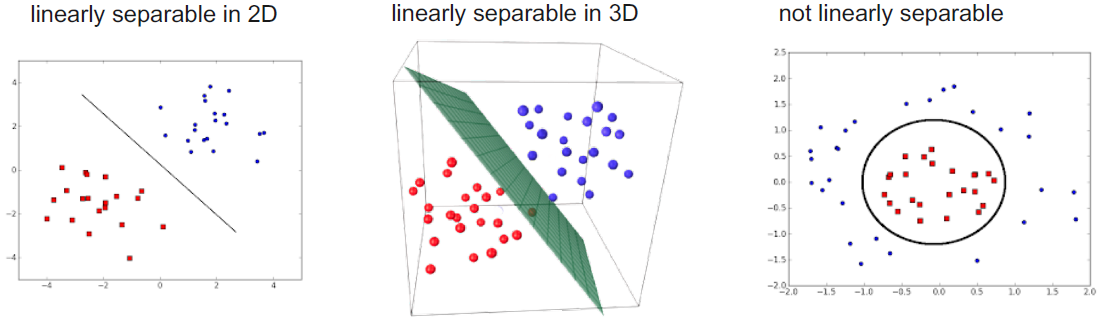
\includegraphics[width=1\linewidth]{linear_sep.png}

\begin{itemize}
    \item Based on logistic regression model, you can draw a line
    \item This is the Linear decision boundary
    \item If a simple line perfectly seperates the classes, then the classes are said to be linear separable
\end{itemize}

\subsection{Non-Linear decision boundary}
\begin{itemize}
    \item When classes are not linearly separable
    \item Resort to polynomial terms
\end{itemize}

\subsection{k-Neares Neighbors (KNN)}
\begin{itemize}
    \item A datapoint is know by the company it keeps
    \item Computes $k$ nearest neighbours
    \item Returns the most frequent class of the $k$ neighbours
\end{itemize}
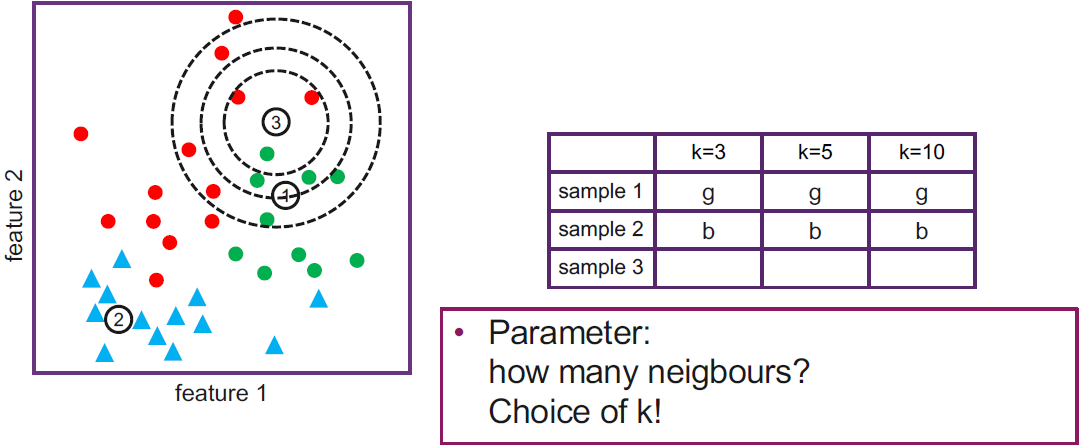
\includegraphics[width=0.8\linewidth]{knn.png}
\textbf{Process}
\begin{enumerate}
    \item Load the training and test data
    \item Choose value of $k$ (number of nearest neighbours to consider for classification)
    \item For each test data points $x_{test}$
        \subitem For all training data $x_{train}$ calculate $d(x_{test}, x_{train})$ with distance metric
        \subitem Sort training data in ascending order of distance
        \subitem Choose first $k$ data points from sorted training data
        \subitem Choose most frequently occurring class from $k$ data points as classification result
\end{enumerate}

\textbf{Distance Metric}
\begin{itemize}
    \item Cosine Distance $cost \theta = \frac{x_1 \cdot x_2}{||x_1|| ||x_2||}$
    \item Manhattan Distance $d_M = \sum_{i=1}^{n}| x_{1,n} - x_{2,n} |$
    \item Euclidean Distance (most used) $d_E = \sqrt{\sum_{i=1n}^{}(x_{1,n} - x_{2,n})^2}$
    \item Minkowski Distance
\end{itemize}

\begin{minipage}[t]{0.5\linewidth}
    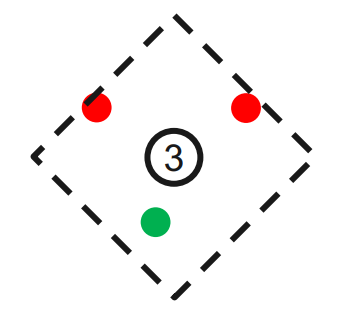
\includegraphics[width=0.6\linewidth]{manhattan-distance.png} \\
    Manhattan Distance
\end{minipage}
\begin{minipage}[t]{0.5\linewidth}
    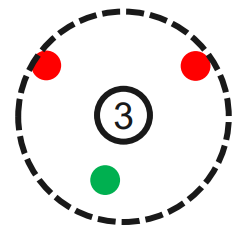
\includegraphics[width=0.6\linewidth]{euclid-distance.png} \\
    Euclidean Distance
\end{minipage}

\textbf{Advantages}
\begin{itemize}
    \item Easy and simple ML model
    \item Few hyperparameters to tune
\end{itemize}

\textbf{Disadvantages}
\begin{itemize}
    \item $k$ should be wisely selected
    \item Large computation cost during runtime if sample size is large
    \item Not efficient for high dimensional datasets
    \item Proper scaling should be provided for fair treatment among features
\end{itemize}

\textbf{Hyperparameters}
\begin{itemize}
    \item \textcolor{blue}{K Value} how many neighbours to participate in the KNN algo.
    \item \textcolor{blue}{Distance Function} Euclidean distance is most used
\end{itemize}
